%=========================================================================
% Start of
%=========================================================================
\preClass{Basic Trigonometry}

\begin{problem}
\item A circle of radius $r$ is centered at the origin, and a ray
  originates from the origin at a given angle, $\theta$. The ray
  passes through the circle at the coordinate $(x,y)$. A function of
  $\theta$ can be defined in terms of the coordinate.

  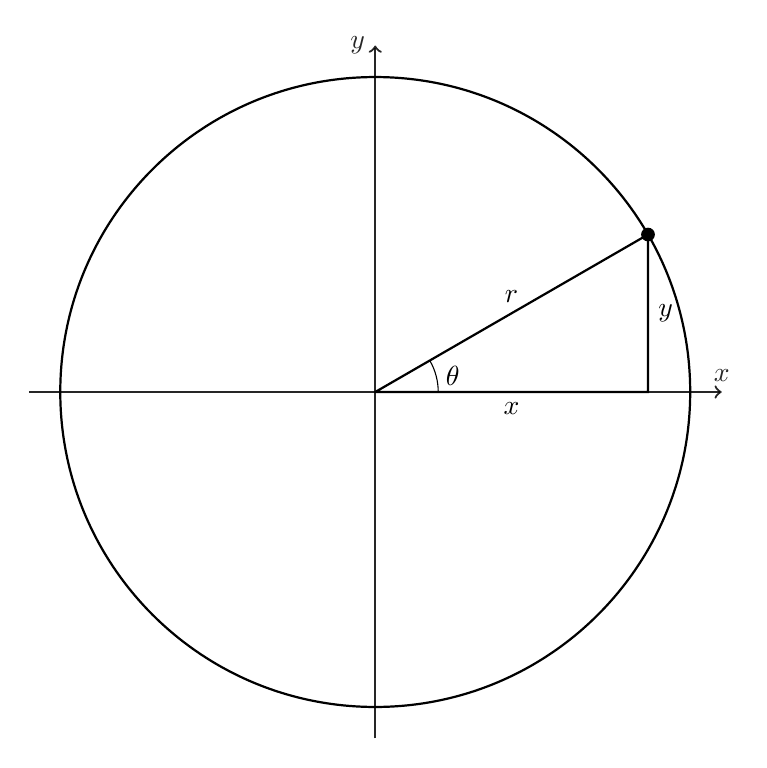
\begin{tikzpicture}[y=4cm, x=4cm,font=\sffamily]
      \draw[thick,opacity=0.85,->] (0, -1.1) -- (0,1.1) node[anchor=east] {$y$};
      \draw[thick,opacity=0.85,->] (-1.1, 0) -- (1.1,0) node[anchor=south] {$x$};
      \draw[thick] (1,0) arc (0:360:1);
      \draw[thick] (0,0) -- (30:1) node[midway,anchor=south] {$r$}
          -- ++(-90:0.5) node[midway,anchor=west] {$y$}
          -- (0,0) node[midway,anchor=north] {$x$};
      \draw[fill=black] (30:1) circle (0.02);
      \draw[text=black] (0:0.2) arc (0:30:0.2) node[midway,anchor=west] {$\theta$};
    \end{tikzpicture}


  \begin{subproblem}
  \item A function, sine, is defined to be
    \begin{eqnarray*}
      \sin(\theta) & = & \frac{y}{r}.
    \end{eqnarray*}
    Determine the formula for the value of $y$ given $r$ and $\theta$
    in terms of the sine function.
    \sideNote{Solve the equation above for $y$.}
    \vfill
  \item A function, cosine, is defined to be
    \begin{eqnarray*}
      \cos(\theta) & = & \frac{x}{r}.
    \end{eqnarray*}
    Determine the formula for the value of $x$ given $r$ and $\theta$
    in terms of the cosine function.
    \sideNote{Solve the equation above for $x$.}
    \vfill
  \end{subproblem}

\end{problem}


\actTitle{Basic Trigonomety}
\begin{problem}
\item Answer each of the following questions where the given point is $P(2,4)$.
  \begin{subproblem}
  \item Make a sketch of the coordinate plane and include the point
    $P(2,4)$. Draw the ray from the origin to the point.
    \sideNote{Label your axes and annotate your plot.}
    \vfill
  \item Add a circle to your sketch show center is the origin and goes
    through the point. Label the angle $\theta$ as the angle between
    the ray and the $x$-axis.
  \item What is the radius of the circle? (Add a label to your plot for the radius.)
    \vspace{2em}
  \item Determine the values of the sine and cosine for the angle.
    \begin{eqnarray*}
      \sin(\theta) & = & \\ [10pt]
      \cos(\theta) & = &
    \end{eqnarray*}
  \end{subproblem}

\clearpage

\item For each point below determine the radius and the value of the
  sine and cosine of the angle associated with each point.
  \begin{subproblem}
  \item $P(1,0)$
    \vfill
  \item $P(0,1)$
    \vfill
  \item $P(-1,0)$
    \vfill
  \item $P(0,-1)$
    \vfill
  \item $P\left(\frac{\sqrt{2}}{2},\frac{\sqrt{2}}{2}\right)$
    \vfill
  \end{subproblem}

\clearpage

\item The circle below is centered at the origin and has a radius of
  one.

  %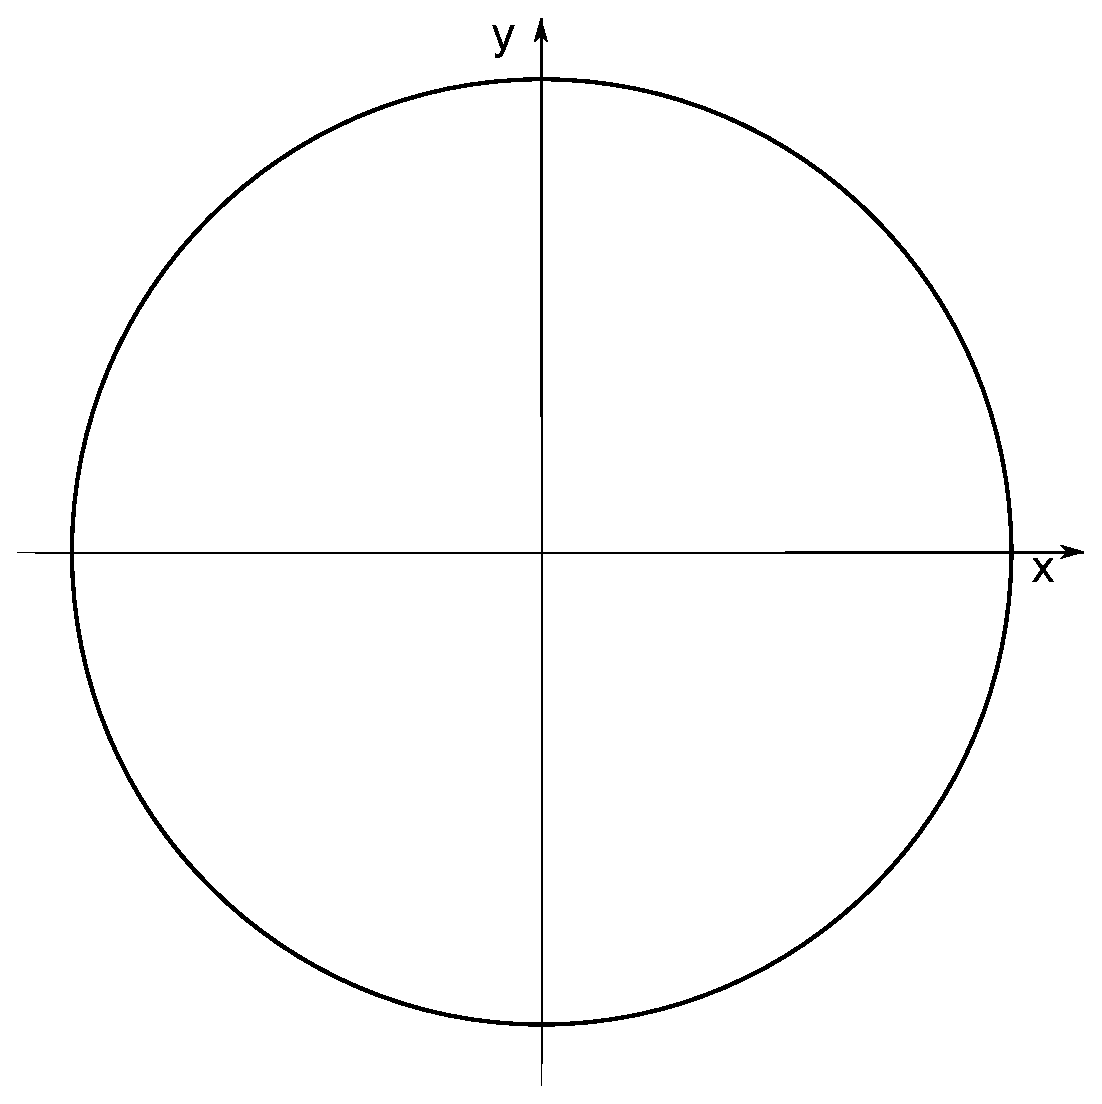
\includegraphics[width=16cm]{trig/img/blankCircle}
  \begin{tikzpicture}[y=6cm, x=6cm,font=\sffamily]
      \draw[thick,opacity=0.85,->] (0, -1.1) -- (0,1.1) node[anchor=east] {$y$};
      \draw[thick,opacity=0.85,->] (-1.1, 0) -- (1.1,0) node[anchor=south] {$x$};
      \draw[thick] (1,0) arc (0:360:1);
    \end{tikzpicture}

  \begin{subproblem}
  \item Mark the locations on the circle whose associated angles are
    0, $\pi/4$, $\pi/2$, $3\pi/4$, $\pi$, $5\pi/4$, $3\pi/2$, and
    $7\pi/4$.
    Determine the coordinates for the points.
    (Label the points and annotate your plot.)
    \clearpage

  \item Determine the $(x,y)$ coordinates for each angle.
    \vfill
  \item Determine the cosine and sine of each angle.
    \vfill
  \end{subproblem}

\end{problem}

\postClass

\begin{problem}
\item Briefly state two ideas from today's class.
  \begin{itemize}
  \item
  \item
  \end{itemize}
\item
  \begin{subproblem}
    \item
  \end{subproblem}
\end{problem}


%%% Local Variables:
%%% mode: latex
%%% TeX-master: "../labManual"
%%% End:
